% !Mode:: "TeX:UTF-8"

\titlepage

\begin{frame}{说在前面}
	\linespread{1.5}
	  \begin{itemize}[<+-|alert@+>]
	    \item \ba{雷同!!!}
	    \item \ba{雷同!!!}
	    \item \ba{雷同!!!}
	  \end{itemize}
\end{frame}

% \begin{frame}{需要注意的问题}
% 	\linespread{1.5}
% 	  \begin{itemize}%[<+-|alert@+>]
% 	    \item L'Hospital法则
% 	    \begin{itemize}
% 	      \item \it 只能应用于“$\df{\bm{0}}{\bm{0}}$”
% 	      和“$\df{\bm{\infty}}{\bm{\infty}}$”型
% 	      \item \it 及时使用无穷小代换进行简化
% 	      \item \it 不正规的符号:\b 
% 	      $\xlongequal{\footnotesize\mbox{“L”}}$、
% 	      $\xlongrightarrow{\footnotesize\mbox{“L'Hospital法则”}}$、
% 	      $\df{\bm{0}}{\bm{0}}$、$\df{\bm{\infty}}{\bm{\infty}}$
% 	    \end{itemize}
% 	    \item Taylor公式
% 	    \begin{itemize}
% 	      \item \it Taylor多项式不包含余项
% 	      \item \it 合并同次幂的系数
% 	      \item \it 尽量按照幂次由低到高排列,最后写余项
% 	    \end{itemize}
% 	  \end{itemize}
% \end{frame}

\section{7.1 概念与应用}

\begin{frame}
	\linespread{1.5}
	\ba{1.请给出如下通解对应的微分方程,并给出其满足给定初值条件的特解:
	
	(1)$y=x^2+C_1x+C_2$,其中$C_1,C_2$为任意常数,$y(0)=y'(0)=1$;}
	
	\bigskip
	
	\small 解:\it
	原方程两边对$x$连续两次求导,可得
	$$y'=2x+C_1,\quad y''=2,$$
	即为所求方程。
	
	将$y(0)=y'(0)=1$分别带入通解和上述第一个方程可得$C_1=C_2=1$,故
	所求特解为$y=x^2+x+1$。
\end{frame}

\begin{frame}
	\linespread{1.5}
	\ba{$y=\df{1+Ce^t}{1-Ce^t}$,其中$C$为任意常数,$y(0)=2$;}
	
% 	\bigskip
	
	\small 解:\it
	原方程可化为
	$$C=\df{y-1}{y+1}e^{-t},$$
	两边对$t$求导,可得
	$$0=\df{2y'-y^2+1}{(y+1)^2}e^{-t},$$
	从而可得
	$$2y'-y^2+1=0,\quad(y\ne-1),$$
	即为所求方程。
	
	将$y(0)=2$带入通解可得$C=\frac13$,从而所求特解为
	$y=\df{3+e^t}{3-e^t}$。
\end{frame}

\begin{frame}
	\linespread{1.5}
	\ba{$y=(C_1+C_2x)e^x$,其中$C_1,C_2$为任意常数,$y(0)=0,y'(1)=1$.}
	
% 	\bigskip
	
	\small 解:\it
	原方程可化为
	$$ye^{-x}=C_1+C_2x,$$
	两边对$x$连续两次求导,可得
	$$(y'-y)e^{-x}=C_2,\quad
	(y''-2y'+y)e^{-x}=0.$$
	因为$e^{-x}\ne0$,故所求方程即为
	$$y''-2y'+y=0.$$
	
	又将$y(0)=0,y'(1)=1$带入通解和前述第一个方程中,可得
	$C_1=0,C_2=\frac1{2e}$,从而所求特解为$y=\frac12xe^{x-1}$。
	\fin
\end{frame}

\begin{frame}
	\linespread{1.5}
	\ba{2.设河边点$O$的正对岸为点$A$,河宽$h$,两岸平行,水流速度恒定为$a$。
	一只鸭子从点$A$游向点$O$,游动过程中其始终朝向$O$点。已知鸭子在
	静水中的游速为$b(b>a)$,以$O$为原点,水流方向为$x$轴,垂直于水流
	过河的方向为$y$轴,试给出鸭子的运动轨迹所满足的微分方程初值问题。}
	
% 	\bigskip

	\begin{center}
		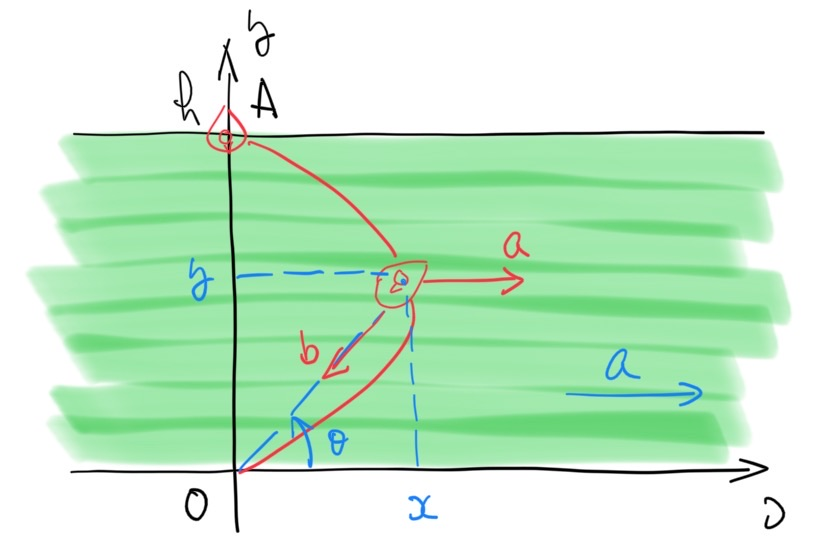
\includegraphics[width=0.6\textwidth]{./images/ch7/duck.jpg}
	\end{center}
\end{frame}

\begin{frame}
	\linespread{1.5}	
	\small 解:\it
	在鸭子运动轨迹上任一点$(x,y)$处,其运动满足
	$$x'_t=a-b\cos\theta,\quad y'_t=-b\sin\theta,$$
	其中
	$$\sin\theta=\df{y}{\sqrt{x^2+y^2}},\quad
	\cos\theta=\df{x}{\sqrt{x^2+y^2}},$$
	故
	$$y'_x=\df{y'_t}{x'_t}=\df{-by}{a\sqrt{x^2+y^2}-bx},$$
	显然$y(0)=h$,故所求初值问题为
	$$
		\left\{\begin{array}{l}
			y'=\df{-by}{a\sqrt{x^2+y^2}-bx},\\
			y(0)=h.
		\end{array}\right.
	$$
	\fin
\end{frame}

\section{7.2 一阶微分方程的解法}

\begin{frame}
	\linespread{1.5}
	\ba{1.求解下列微分方程:
	
	(1)$xy'-y+\sqrt{x^2-y^2}=0,(x>0)$}
	
	\bigskip
	
	\small 解:\it
	令$z=\frac yx$,则原方程可化为
	$$xz'+\sqrt{1-z^2}=0.$$
	当$\sqrt{1-z^2}\ne 0$时,该方程分离变量,解得$z=\sin(-\ln x+C)$。
	当$\sqrt{1-z^2}=0$时,方程有解$y=\pm x$。
	
	综上,原方程的解为
	$$y=x\sin(\ln x+C),\;(x\in\mbb{R})
	\quad\mbox{或}\quad y=\pm x.$$
\end{frame}

\begin{frame}
	\linespread{1.5}
	\ba{(2)$y'=(x+y)^2$}
	
	\bigskip
	
	\small 解:\it
	令$z=x+y$,则原方程可化为
	$$z'-1=z^2,$$
	该方程分离变量,解得$z=\tan(x+C)$,进而原方程的解为
	$$x+y=\tan(x+C),\;(C\in\mbb{R}).$$
\end{frame}

\begin{frame}
	\linespread{1.5}
	\ba{(3)$x\ln x\d y+(y-\ln x)\d x=0$ }
	
	\bigskip
	
	\small 解:\it
	令$u=\ln x$,则原方程可化为
	$$u\d y+(y-u)\d u=0,$$
	该方程是一个齐次方程(也是一个全微分方程),可解得
	$2yu-u^2=C$,故原方程的解为
	$$(2y-\ln x)\ln x=C,\;(C\in\mbb{R}).$$
\end{frame}

\begin{frame}
	\linespread{1.5}
	\ba{(4)$3y'+y=(1-x)y^4$}
	
	\bigskip
	
	\small 解:\it
	该方程为Bernoulli方程。当$y\ne0$时,令
	$z=y^{-3}$,则原方程可化为
	$$-z'+z=1-x,$$
	该方程为一阶非齐次线性微分方程,可解得
	$z=-x+Ce^x$。显然$y=0$是方程的特解。综上原方程的解为
	$$y^3(-x+Ce^x)=1,\;(C\in\mbb{R}),\;\mbox{或}\;y=0.$$
	\fin
\end{frame}

\begin{frame}
	\linespread{1.5}
	\ba{2.某湖泊的水量为$V$,每年排入湖内的污水和净水量均为$V/6$,且湖内的总水量不变。
	已知1999年底湖内的污染物含量为$5m_0$。为了治理污染,从2000初开始,限定排入
	湖中的污水中污染物浓度不得超过$m_0/V$。问至少需要经过多少年,
	湖内的污染物含量能够降至$m_0$以下?(注:假设湖水中的污染物浓度是均匀分布的。)}
	
	\bigskip
	
	\small 解:\it
	设$m(t)$为自2000年起第$t$年时湖内的污染物总量,则
	$$m'=\df{m_0}6-\df{m}3,$$
	且$m(0)=5m_0$。
\end{frame}

\begin{frame}
	\linespread{1.5}
	\small\it
	
	设$m(t)$为自2000年起第$t$年时湖内的污染物总量,则
	$$m'=\df{m_0}6-\df{m}3,$$
	且$m(0)=5m_0$。解之可得
	$$m=\df{m_0}2\left(1+9e^{-\frac13t}\right).$$
	令$m<m_0$,可得$t>3\ln9\approx6.59$,故大约7年后,湖水中的污染物含量可以
	降至$m_0$以下。\fin
\end{frame}

\begin{frame}
	\linespread{1.5}
	\ba{3.已知$f(0)=0,f(1)=1$,且当$x\in(0,1)$时,$f''(x)<0$。任取曲线
	$y=f(x)$上一点$(x,f(x)),\;(x\in(0,1))$,该点与原点的连线与曲线所围图形
	面积为$x^2$,求$f(x)$。}
	
	\begin{center}
		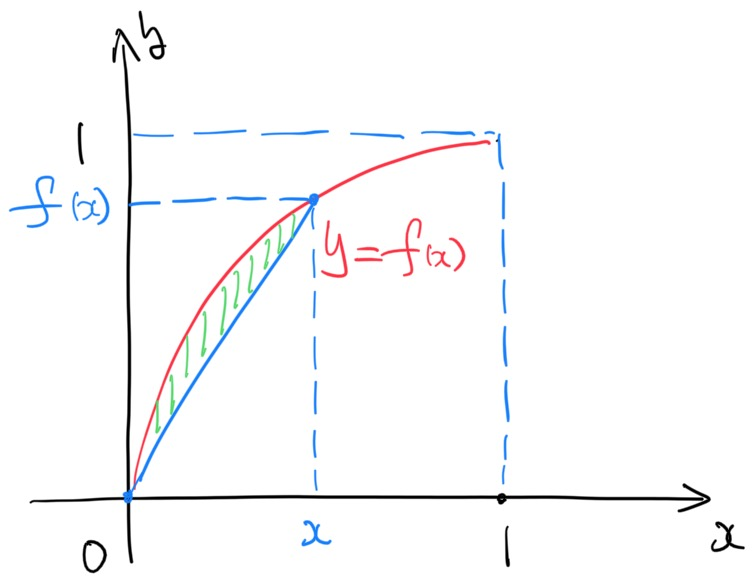
\includegraphics[width=0.6\textwidth]{./images/ch7/fxx2.jpg}
	\end{center}
\end{frame}

\begin{frame}
	\linespread{1.5}	
	\small 解:\it
	由已知
	$$\dint_0^xf(t)\d t-\df12xf(x)=x^2,\quad x\in[0,1],$$
	两边求导,整理得
	$$f(x)-xf'(x)=4x.$$
	该方程为一阶非齐次线性微分方程,解之得
	$$f(x)=(-4\ln x+C)x,\;(C\in\mbb{R},x\in(0,1)),$$
	带入$f(1)=1$,可解得$C=1$,从而所求曲线的方程为
	$$f(x)=\left\{\begin{array}{ll}
		0,& x=0,\\
		(-4\ln x+1)x,& x\in(0,1].
	\end{array}\right.$$
	\fin
\end{frame}

\begin{frame}
	\linespread{1.5}
	\ba{4.某学生将乘积的导数公式错误地记作$(fg)'=f'g'$,然而在一次求导时居然
	得到了正确的结果。目前知道他使用的$f(x)=e^{x^2}\,(x>1/2)$,
	问他用到的$g(x)$可能是什么?}
	
	\bigskip
	
	\small 解:\it
	由已知
	$$(e^{x^2}g(x))'=(e^{x^2})'g'(x),$$
	展开化简可得
	$$2xg=(2x-1)g',$$
	该方程分离变量,求解可得
	$$g(x)=Ce^x\sqrt{2x-1},\;(x>\frac12).$$
	\fin
\end{frame}

% \begin{frame}{出现的问题}
% 	\linespread{1.5}
% 	  \begin{itemize}%[<+-|alert@+>]
% 	    \item 作业进度慢!
% 	    \item 概念问题
% 	    \begin{itemize}
% 	      \item \b\it 幂级数展开不熟练
% 	      \item \b\it Maclaurin级数和关于$(x-x_0)$的幂级数分不清
% 	    \end{itemize}
% 	    \item 过程不规范或不完整
% 	    \begin{itemize}
% 	      \item \b\it 求收敛域要单独讨论端点的敛散性
% 	      \item \b\it 相同幂次的项要合并,并按幂次从小到大排列
% 	      \item \b\it 书写潦草随意\pause
% 	    \end{itemize}
% 	    \item \ba{雷同!!!}
% 	  \end{itemize}
% \end{frame}

% \begin{frame}
% 	\linespread{1.5}
% 	\ba{3.设$D$是由曲线$y=\sin x+1$与三条直线$x=0,x=\pi,y=0$
% 	所围成的曲边梯形,求$D$绕$x$轴旋转一周所围成的旋转体的体积。
% 	}
% 	\pause
% 	
% % 	\bigskip
% 	
% 	\begin{columns}
% 		\begin{column}{.5\textwidth}
% 			\begin{center}
% 				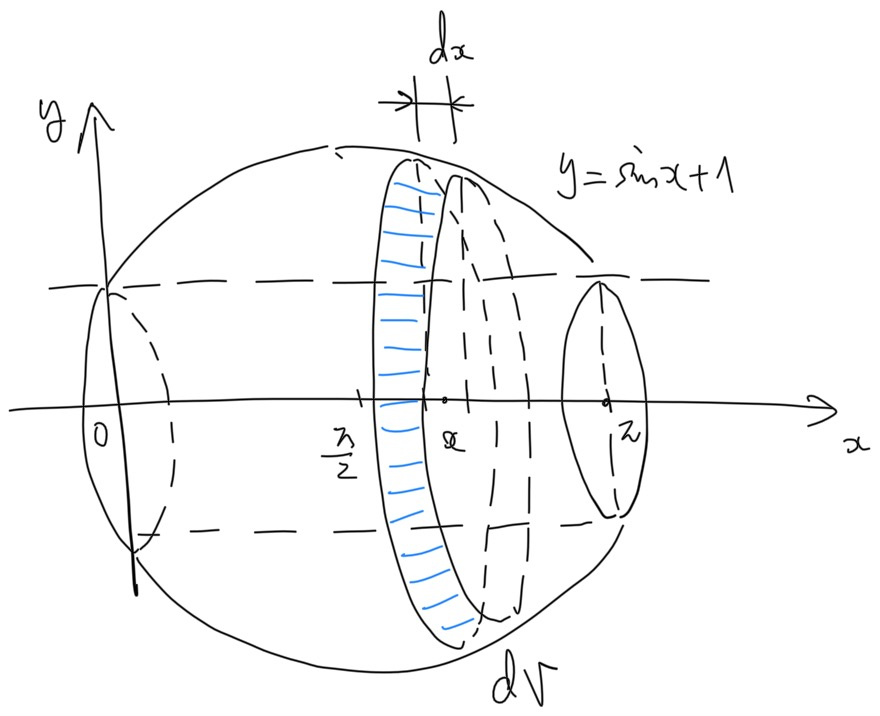
\includegraphics[width=.9\textwidth]{./images/ch6/sinx1cs.jpg}
% 		% 		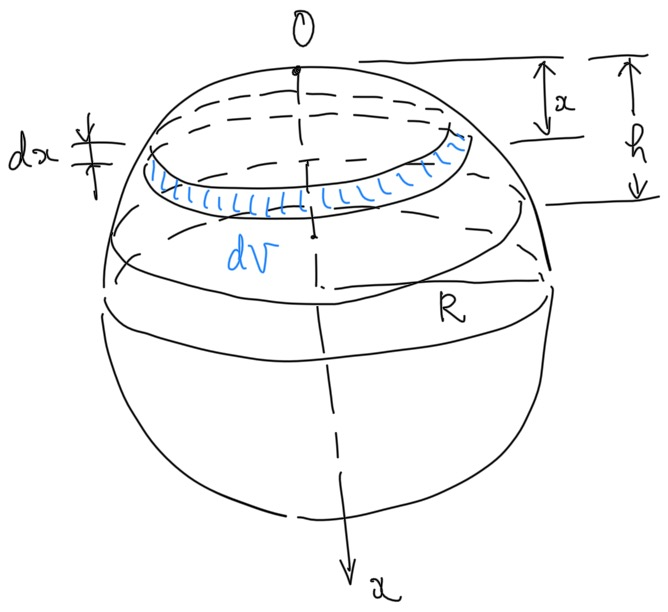
\includegraphics[width=6cm]{./images/ch6/topSp.jpg}
% 			\end{center}		
% 		\end{column}
% 		\begin{column}{.5\textwidth}
% 			\small 解:\it
% 			如图,体积微元$\d V=\pi y^2\d x$,	故所求体积
% 			$$
% 				V=\dint_0^{\pi}\pi(\sin x+1)^2\d x=\df32\pi^2.
% 			$$
% 		\end{column}
% 	\end{columns}
% \end{frame}